
\de{ĐỀ THI HỌC KỲ I NĂM HỌC 2022-2023}{THPT Tam Phú}


\begin{bt}%[Dự án đề kiểm tra HKII NH22-23 - Nguyên Huỳnh]%[THPT Tam Phú]%[0T3B1-2] 
	Tìm tập xác định của hàm số $y = \sqrt{4x-2} + \sqrt{5-2x}$.
	\loigiai{Điều kiện xác định $\heva{&4x-2\ge 0\\&5-2x\ge 0}\Leftrightarrow \heva{&x\ge \dfrac{1}{2}\\&x\le \dfrac{5}{2}.} \Leftrightarrow \dfrac{1}{2}\le x\le \dfrac{5}{2}$
		\\Vậy tập xác định của hàm số là $\mathscr D = \left[ \dfrac{1}{2}; \dfrac{5}{2} \right]$.
	}
	
\end{bt}

\begin{bt} %[Dự án đề kiểm tra HKII NH22-23 - Nguyên Huỳnh]%[THPT Tam Phú]%[0T3B1-5]  
	\immini{	Cho hàm số $y = f(x)$ có đồ thị trên $[-2; 3]$ như sau. 	\begin{enumerate}
			\item[a)] Lập bảng biến thiên của hàm số trên $[-2; 3]$.
			\item[b)] Cho biết giá trị lớn nhất và giá trị nhỏ nhất của hàm số trên $[0; 3]$.
	\end{enumerate}}
	{
		\begin{tikzpicture}[line join = round, line cap = round,>=stealth,font=\footnotesize,scale=0.7]
			\def\xt{-3} \def\xp{4} \def\yd{-4} \def\yt{3} ;
			\draw[->] (\xt,0)--(\xp,0) node[above]{$x$};
			\draw[->] (0,\yd)--(0,\yt) node[left]{$y$};
			\draw[dashed,thin,black] (-2,0)--(-2,2)--(0,2);
			\draw[dashed,thin,black] (0,1)--(1,1)--(1,0);
			\draw[dashed,thin,black] (3,0)--(3,-3)--(0,-3);
			\fill (0,0) circle (1.5pt) node[below left]{$O$} (-2,0) circle (1.5pt) node[below]{$-2$} (-1,0) circle (1.5pt)  (1,0) circle (1.5pt) node[below]{$1$} (2,0) circle (1.5pt) node[below left]{$2$} (3,0) circle (1.5pt) node[above]{$3$} (0,-3) circle (1.5pt) node[left]{$-3$} (0,-1) circle (1.5pt) node[left]{$-1$} (0,1) circle (1.5pt) node[left]{$1$} (0,2) circle (1.5pt) node[right]{$2$};
			\begin{scope}
				\clip (-2,0) rectangle (0,2);
				\draw[samples=150,thick,smooth,domain=\xt:\xp] plot(\x,{-\x});
			\end{scope}
			\begin{scope}
				\clip (0,-3) rectangle (3,1);
				\draw[samples=150,thick,smooth,domain=\xt:\xp] plot(\x,{-(\x)^2 + 2*\x});
			\end{scope}
		\end{tikzpicture}
	}
	
	\loigiai{
		\begin{enumerate}
			\item[a)] Ta có bảng biến thiên của hàm số $y = f(x)$ trên $[-2; 3]$ như sau
			\begin{center}
				
\begin{tikzpicture}[line join = round, line cap = round,>=stealth,font=\footnotesize,scale=1]
					\tkzTabInit[nocadre=false,lgt=1,espcl=2.5,deltacl=0.5]{$x$/1,$y$/2}
					{$-2$ , $0$ , $1$ , $3$}
					\tkzTabVar{+/$2$ , -/$0$ , +/$1$ , -/$-3$}
				\end{tikzpicture}
			\end{center}
			\item[b)] Trên đoạn $[0; 3]$ giá trị lớn nhất của hàm số là 2, giá trị nhỏ nhất của hàm số là $-3$.
		\end{enumerate}
	}
\end{bt}

\begin{bt}%[Dự án đề kiểm tra HKII NH22-23 - Nguyên Huỳnh]%[THPT Tam Phú]%[0T3B2-4] 
	Cho hàm số $y = 2x^{2} + 4x - 1$ có đồ thị $(P)$.
	\begin{enumerate}
		\item[a)] Vẽ đồ thị $(P)$.
		\item[b)] Tìm tọa độ giao điểm của $(P)$ và đường thẳng $d: y = -x - 3$.\dapso{$\left( -\dfrac{1}{2}; -\dfrac{5}{2} \right)$ và $\left( -2; -1 \right)$}
	\end{enumerate}
	\loigiai{	\begin{enumerate}
			\item[a)] Ta có đồ thị của $(P)$ như sau 
			\begin{center}
				\begin{tikzpicture}[line join = round, line cap = round,>=stealth,font=\footnotesize,scale=1]
					\def\a{2}
					\def\b{4}
					\def\c{-1}
					\def\f(#1){\a*((#1)^2)+\b*(#1)+\c}
					\pgfmathsetmacro\ct{-\b/(2*\a)}
					\def\xmin{-2.5}
					\def\xmax{0.5}
					\def\ymin{-3}
					\def\ymax{1}
					\draw[->] (\xmin-1,0)--(\xmax+1,0) node[below] { $x$};
					\draw[->] (0,\ymin-1)--(0,\ymax+1) node[left] { $y$};
					\draw (0,0) node [below left] { $O$};
					\foreach \x in {-3,-2,-1,1}		\draw (\x,0.1)--(\x,-0.1) node [above] { $\x$};
					%	\foreach \y in {-3,-2,-1,1,2,3}		\draw (0.1,\y)--(-0.1,\y) node [left] { $\y$};
					%	\clip (\xmin,\ymin) rectangle (\xmax,\ymax);
					\draw[thick,smooth,samples=200] plot[domain=\xmin:\xmax] (\x,{\f(\x)});
					\draw[dashed] (\ct,0)--(\ct,{\f(\ct)})--(0,{\f(\ct)});
					\draw (-1,-3.5)--(-1,1.8);
					\fill (\ct,{\f(\ct)}) circle (1pt);
					\draw (\xmax,{\f(\xmax)}) node [above right]{$2x^2+4x-1$};
				\end{tikzpicture}
			\end{center}
			\item[b)] Phương trình hoành đồ giao điểm của $(P)$ và $(d)$ là 
			\begin{eqnarray*}
				2x^2+4x-1=-x-3 &\Leftrightarrow & 2x^2+5x+2=0 \\&\Leftrightarrow & \hoac{&x=-\dfrac{1}{2}\\& x=-2.} 
			\end{eqnarray*}
			Khi đó, tọa độ giao điểm của $(P)$ và $(d)$ là $\left( -\dfrac{1}{2}; -\dfrac{5}{2} \right)$ và $\left( -2; -1 \right)$.
		\end{enumerate}
	}
\end{bt}

\begin{bt}%[Dự án đề kiểm tra HKII NH22-23 - Nguyên Huỳnh]%[THPT Tam Phú]%[0T4B3-1]
	Cho tam giác $ABC$ biết $CA=8{,}2$ và $\widehat{C}=110^{\circ}, \widehat{B} = 25^{\circ}$. Tính độ dài cạnh $BC$ và diện tích tam giác $ABC$. \dapso{$BC \approx 13{,}7, \enskip S_{ABC} \approx 52{,}9 $}
	\loigiai{Do $\widehat A+\widehat B+\widehat C=180^\circ$ nên $\widehat A=45^\circ$.\\
		Áp dụng định lý sin ta có 
		$$\dfrac{BC}{\sin A}=\dfrac{CA}{\sin B}\Rightarrow BC=\dfrac{CA\cdot\sin A}{\sin B}\approx 13{,}72.$$
		Ta có $S_{ABC}=\dfrac{1}{2}CA\cdot CB\cdot\sin C\approx\dfrac{1}{2}8{,}2\cdot13{,}72 \cdot\sin 110^\circ\approx52{,}86$.
	}
\end{bt}

\begin{bt}%[Dự án đề kiểm tra HKII NH22-23 - Nguyên Huỳnh]%[THPT Tam Phú]%[0T4N3-1]
	Cho tam giác $ABC$ có $AB = 5; BC = 9; \widehat{ABC} = 30^{\circ}$. Tính $\overrightarrow{AB}\cdot\overrightarrow{BC}$. \loigiai{Ta có $\overrightarrow{AB}\cdot\overrightarrow{BC}=-\overrightarrow{BA}\cdot\overrightarrow{BC}=-BA\cdot BC\cdot \cos(\overrightarrow{BA},\overrightarrow{BC})=-5\cdot 9\cdot \cos30^\circ=-\dfrac{45\sqrt3}{2}$.
	}
	
\end{bt}


%[Câu 6]
\begin{bt}%[0T5K2-5]%[Dự án đề kiểm tra HKI NH22-23 Lê Hùng Thắng]%[TRƯỜNG THPT TAM PHÚ - HCM]
	Cho tam giác $ABC$ vuông cân đỉnh $C$ biết $AB = 4\sqrt{2}$. Tính $\left| \overrightarrow{AB} + \overrightarrow{AC} \right|$. \dapso{$4\sqrt{5}$}
\loigiai{
\immini{Tam giác $ABC$ vuông cân tại $C$ nên $AC=BC=\dfrac{AB}{\sqrt{2}}=4$.\\
Gọi $I$ là trung điểm của $BC$, ta có\\
$\vec{AB}+ \vec{AC}=2 \vec{AI} \Rightarrow |\vec{AB}+ \vec{AC}|=2 |\vec{AI}|=2 AI$.\\
Mà $AI=\sqrt{AC^2+CI^2}=\sqrt{4^2+2^2}=2\sqrt{5}$.\\
Vậy $|\vec{AB}+ \vec{AC}|=4\sqrt{5}$.
}
{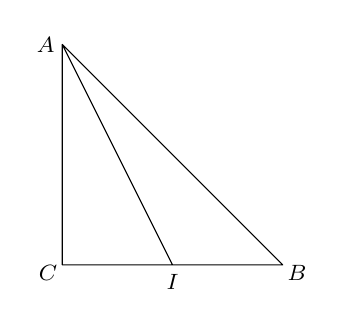
\begin{tikzpicture}[scale=0.7,>=stealth, font=\footnotesize, line join=round, line cap=round]
\path (0,0) coordinate (C) 
 (4,0) coordinate (B) 
 (0,4) coordinate (A) 
 (2,0) coordinate (I);
 \draw (I)--(A)--(B)--(C)--(A);
\tkzMarkRightAngles[size=0.3](B,C,A)
\foreach \d/\g in {A/180,B/-30,C/-150,I/-90} \fill (\d) ++ (\g:3mm) node {$\d$};
	\end{tikzpicture}
}
}
\end{bt}
%[Câu 7]
\begin{bt}%[0T5B4-1]%[Dự án đề kiểm tra HKI NH22-23 Lê Hùng Thắng]%[TRƯỜNG THPT TAM PHÚ - HCM]
	Tính $ \cos \left(\vec{a},\vec{b}\right) $ biết $ \lvert\vec{a}\rvert=20 $, $ \lvert\vec{b}\rvert=160 $ và $ \vec{a}\cdot \vec{b}=-80 $. \dapso{$\dfrac{-1}{40}$}
\loigiai{Ta có $$\cos(\vec{a},\vec{b})
	=\dfrac{\vec{a}\cdot \vec{b}}{|\vec{a}|\cdot |\vec{b}|} 
	= \dfrac{-80}{20 \cdot 160}= \dfrac{-1}{40}.$$
	}
\end{bt}

%[Câu 8]
\begin{bt}%[0T3K2-5]%[Dự án đề kiểm tra HKI NH22-23 Lê Hùng Thắng]%[TRƯỜNG THPT TAM PHÚ - HCM]
\immini [thm]{Trong lúc chơi bóng rổ, bạn Bình phát hiện ra quỹ đạo ném xiên của quả bóng là một parabol. Trong một lần ném, quả bóng đạt độ cao $3$ m tại điểm $A$ và tiếp tục đạt vị trí cao nhất so với mặt đất là $5$ m tại điểm $I$. Gọi $O,H$ lần lượt là chân đường vuông góc của $A$ và $I$ lên mặt đất ($AO=3$ m, $IH=5$ m). Biết $OH=3$ m (tham khảo hình vẽ).
}
{\begin{tikzpicture}[scale=0.75,>=stealth, font=\footnotesize, line join=round, line cap=round]
	\def\a{-2/9}
	\def\b{4/3}
	\def\c{3}
	\def\f(#1){\a*((#1)^2)+\b*(#1)+\c}
	\pgfmathsetmacro\ct{-\b/(2*\a)}
	\def\xmin{0}
	\def\xmax{5.5}
	\def\ymin{0}
	\def\ymax{6}
	\draw[-] (\xmin-1,0)--(6,0);
	\path (0,0) coordinate (O)
	(0,3) coordinate (A)
	(3,0) coordinate (H)
	(3,5)coordinate (I)
	(5,0) coordinate (D)
	(5,3) coordinate (M);
%	\foreach \x in {O,A,H,I,M,D} \node[below left] at (\x) {$\x$};
	\foreach \d/\g in {A/180,O/-90,H/-90,D/-90,M/0,I/45} \fill (\d) ++ (\g:3.5mm) node {$\d$};
	\draw[<->] ($(O)+(0,0.3)$) -- ($(H)+(0,0.3)$) node[above,sloped,pos=0.5] {$3$ m};
	\draw[<->] ($(O)+(0,-0.6)$) -- ($(D)+(0,-0.6)$) node[below,sloped,pos=0.5] {$5$ m};
%	\draw (A)--(B) node[below,sloped,pos=0.5] {m};
	\draw[<->] (O) --(A) node[above,sloped,pos=0.5] {$3$ m};
	\draw[<->] (H) --(I) node[above,sloped,pos=0.5] {$5$ m};
	\draw[<->] (D) --(M) node[above,sloped,pos=0.5] {$3$ m};
%	\draw[<->] (O) --(D) node[above,sloped,pos=0.5] {$5$ m};
	\clip (\xmin,0) rectangle (\xmax,\ymax);
	\draw[smooth,samples=200] plot[domain=\xmin:4] (\x,{\f(\x)});
	\end{tikzpicture}
}
	\begin{enumerate}
	\item Nếu chọn điểm $ O $ làm gốc tọa độ, em hãy giúp bạn Bình lập phương trình quỹ đạo của quả bóng khi đó. \dapso{$y=-\dfrac{2}{9}x^2+\dfrac{4}{3}x+3$}
	\item Trong mặt phẳng quỹ đạo của quả bóng, nếu tâm rổ đặt tại vị trí điểm $ M $ cách mặt đất $ 3$ m. $D$ là chân đường vuông góc của $M$ lên mặt đất và $ OD=5$ m thì trái bóng bạn Bình ném như trên có vào rổ không? Tại sao? \dapso{Không}
	\end{enumerate}
\loigiai{
\begin{enumerate}
	\item Chọn điểm $ O $ làm gốc tọa độ, $OD$ là trục hoành và $OA$ là trục tung. Khi đó $A(0;3)$, $I(3;5)$.\\
	Gọi phương trình của parabol có dạng $(P)\colon y=ax^2+bx+c$, $a\ne 0$.\\
	Vì $(P)$ qua $A(0;3)$ và có đỉnh là $I(3;5)$ nên ta có\\
	$\heva{& \dfrac{-b}{2a}=3\\& 9a+3b+c=5 \\&c=3} \Leftrightarrow \heva{&a=\dfrac{-2}{9} \\&b= \dfrac{4}{3}\\& c=3.}$\\
	Vậy $(P)\colon y=\dfrac{-2}{9}x^2+\dfrac{4}{3}x+3$.
	 \dapso{$y=-\dfrac{2}{9}x^2+\dfrac{4}{3}x+3$}
	\item Theo đề ra ta có $M(5;3)$.\\
	Vì $M \notin (P)$ nên theo cách ném trên thì quả bóng không đi vào rổ.	
\end{enumerate}
}
\end{bt}

%[Câu 9]
\begin{bt}%[0T4B3-1]%[Dự án đề kiểm tra HKI NH22-23 Lê Hùng Thắng]%[TRƯỜNG THPT TAM PHÚ - HCM]
\immini [thm]{	Một công ty du lịch lữ hành mở hai tuyến đường du lịch từ vị trí $ A $ đến vị trí $ B $. Tuyến thứ nhất, đi từ $ A $ đến $ B $ bằng phương tiện cáp treo. Tuyến thứ hai, họ muốn đi bộ từ $ A $ đến $ C $ rồi mới dùng cáp treo đi từ $ C $ đến $ B $. Tính độ dài cáp treo từ $ C $ đến $ B $ biết chiều dài cáp treo từ $ A $ đến $ B $ là $1672$ m, quãng đường người du lịch đi bộ từ $ A $ đến $ C $ là $ 950 $ m và $ \widehat{BAC}=32^\circ $.
}
{\begin{tikzpicture}
	\path 	(0,0) coordinate (A)
	(3,0) coordinate (C)
	(4,3) coordinate (B);
	\draw (A) -- (B) node[above,sloped,pos=0.5] {$1672$ m};
	\draw (B)--(C) (A) -- (C) node[below,sloped,pos=0.5] {$950$ m};
	\draw pic["$32^{\circ}$",angle eccentricity=1.5,draw,angle radius=0.7cm]{angle=C--A--B};
	\foreach \d/\g in {A/180,B/0,C/0} \fill (\d) ++ (\g:3mm) node {$\d$};
	\end{tikzpicture}
}
 \dapso{$1002$}
\loigiai
{Xét tam giác $ABC$ ta có\\
	\allowdisplaybreaks
	$\begin{aligned}[t]
	BC^2= & AB^2+AC^2-2\cdot AB \cdot AC \cdot \cos \widehat{BAC}\\
	= & 1672^2+950^2 -2 \cdot 1672 \cdot 950 \cdot \cos 32^\circ \\
\approx & 1004004{,}808.
	\end{aligned}$ \\
Vậy $BC \approx 1002$ m.
}
\end{bt}

